\documentclass[11pt, twoside, pdftex]{article}

% This includes all the settings that we should use for the document
\newcommand{\PDFTitle}{Accessing HPS Devices from the FPGA}
\newcommand{\commonPath}{../../Common}
\newcommand{\datePublished}{Mar 2022}

\newcommand{\versnum}{21.1} %version number quartus/AMP
\newcommand{\quartusname}{Quartus\textsuperscript{\textregistered} Prime}	
\newcommand{\textBar}{For \quartusname{} \versnum{}}
\newcommand{\thisyear}{2022 } %for copyright
\newcommand{\company}{FPGAcademy.org}
\newcommand{\longteamname}{FPGAcademy.org}
\newcommand{\teamname}{FPGAcademy}
\newcommand{\website}{FPGAcademy.org}

\newcommand{\productAcronym}{AMP}
\newcommand{\productNameShort}{Monitor Program}

\newcommand{\productNameMedTM}{Monitor Program}
\newcommand{\productNameMed}{Monitor Program}

%\newcommand{\headerLogoFilePath}[1]{#1/FPGAcademy.png}



\setlength\topmargin{-0.25in}
\setlength\headheight{0in}
\setlength\headsep{0.35in}
\setlength\textheight{8.5in}
\setlength\textwidth{7in}
\setlength\oddsidemargin{-0.25in}
\setlength\evensidemargin{-0.25in}
\setlength\parindent{0.25in}
\setlength\parskip{0in} 

\pdfpagewidth 8.5in
\pdfpageheight 11in

% listings is a package that supports encapsulating source code in LaTeX conveniently

\usepackage{listings}
% add support for graphics
\usepackage{graphicx}
\usepackage[usenames, dvipsnames]{color}

\def\expandparam\lstinputlisting[#1]#2{\edef\tmp{\noexpand\lstinputlisting[#1]{#2}}\tmp}

\widowpenalty 10000
\clubpenalty 10000

%%%%%%%%%%%%%%%%%%%% Source Code Formatting %%%%%%%%%%%%%%%%%%%%
\definecolor{globalCommentColour}{rgb}{0.588,0.588,0.588}

%%%%%%%%%%%%%%%%%%%%%%%%%%%%%%%%%%%%%%%%%%%%%%%%%%%%
% Defining a NiosII ASM highlighter for lstlisting
\lstdefinelanguage[NiosII]{Assembler} {
 	morekeywords={add, addi, and, andhi, andi, beq, bge, bgeu, bgt, bgtu, ble,  bleu, blt, bltu, bne, br, break,% 
 	bret, call, callr, cmpeq, cmpeqi, cmpge, cmpgei, cmpgeu, cmpgeui, cmpgt, cmpgti, cmpgtu, cmpgtui, cmple,%
 	cmplei, cmpleu, cmpleui, cmplt, cmplti, cmpltu, cmpltui, cmpne, cmpnei, custom, div, divu, eret, flushd,%
 	flushda, flushi, flushp, initd, initda, initi, jmp, jmpi, ldb, ldbio, ldbu, ldbuio, ldh, ldhio, ldhu, ldhuio,%
 	ldw, ldwio, mov, movhi, movi, movia, movui, mul, muli, mulxss, mulxsu, mulxuu, nextpc, nop, nor, or, orhi, ori,%
 	rdctl, rdprs, ret, rol, roli, ror, sll, slli, sra, srai, srl, srli, stb, stbio, sth, sthio, stw, stwio,%
 	sub, subi, sync, trap, wrctl, wrtcl, wrprs, xor, xori, xorhi, xori},% 	
 	morekeywords=[2]{.abort, .ABORT, .align, .app-file, .ascii, .asciz, .balign, .byte, .comm, .data, .def,%
 	.desc, .dim, .double, .eject, .else, .end, .endef, .endif, .equ, .equiv, .err, .extern, .file, .fill, .float,%
 	.global, .globl, .hword, .ident, .if, .include, .int, .irp, .irpc, .lcomm, .lflags, .line, .linkonce, .ln,%
 	.list, .long, .macro, .mri, .nolist, .octa, .org, .p2align, .psize, .quad, .rept, .sbttl, .scl, .section,%
 	.set, .short, .single, .size, .sleb128, .skip, .space, .stadb, .stabn, .stabs, .string, .symver, .tag,%
 	.text, .title, .type, .val, .uleb128, .word},% 	
 	morekeywords=[3]{et, bt, gp, sp, fp, ea, sstatus, ra, pc, status, estatus, bstatus, ienable, ipending, cpuid,%
 	exception, pteaddr, tlbacc, tlbmisc, eccinj, badaddr, config, mpubase, mpuacc},% 	
 	sensitive=t,%
 	alsoletter=.,%
	morestring=[b]",%
 	morecomment=[s]{/*}{*/},%
 	morecomment=[l]\#,%
   }[keywords,comments,strings]
   
   %% NOTE: morekeywords=[2] are GNU directives.
   
   \definecolor{niosInstructionColour}{rgb}{0.000,0.608,0.000}
   \definecolor{niosDirectiveColour}{rgb}{0.000,0.000,0.902}
   \definecolor{niosSpecialRegColour}{rgb}{0.000,0.000,0.000}
   \definecolor{niosStringColour}{rgb}{0.808,0.482,0.000}
   
   %% NOTE: To make bold use: =\bfseries\color{<colour>}
   \lstdefinestyle{defaultNiosStyle} {
   language=[NiosII]{Assembler},
   stringstyle=\color{niosStringColour},
   keywordstyle=\color{niosInstructionColour},
   keywordstyle=[2]\color{niosDirectiveColour},
   keywordstyle=[3]\itshape\color{niosSpecialRegColour}
   }
%%%%%%%%%%%%%%%%%%%%%%%%%%%%%%%%%%%%%%%%%%%%%%%%%%%%

%%%%%%%%%%%%%%%%%%%%%%%%%%%%%%%%%%%%%%%%%%%%%%%%%%%%
% Defining a ArmA9 ASM highlighter for lstlisting
\lstdefinelanguage[ArmA9]{Assembler} {
 	morekeywords={ADC, ADD, ADDS, AND, ANDS, B, BAL, BEQ, BGE, BGT, BL, BLT, BIC, BKPT, BLX, BNE, BX, CDP, CLZ, CMN, CMP, EOR,%
 	EORS, LDC, LDM, LDR, LDRB, LDRBT, LDRH, LDRSB, LDRSH, LDRT, LSL, MCR, MLA, MOV, MOVW, MOVT, MRC, MRS, MSR, MUL, MVN, ORR, PLD,%
 	ROR, RSB, RSC, SBC, SMLAL, SMULL, STC, STM, STR, STRB, STRBT, STRH, STRT, SUB, SUBS, SWI, SWP, SWPB, TEQ, UMLAL,
 	PUSH, POP, MOVS, RORS, LSR},%
 	morekeywords=[2]{.abort, .ABORT, .align, .app-file, .ascii, .asciz, .balign, .byte, .comm, .data, .def,%
 	.desc, .dim, .double, .eject, .else, .end, .endef, .endif, .equ, .equiv, .err, .extern, .file, .fill, .float,%
 	.global, .globl, .hword, .ident, .if, .include, .int, .irp, .irpc, .lcomm, .lflags, .line, .linkonce, .ln,%
 	.list, .long, .macro, .mri, .nolist, .octa, .org, .p2align, .psize, .quad, .rept, .sbttl, .scl, .section,%
 	.set, .short, .single, .size, .sleb128, .skip, .space, .stadb, .stabn, .stabs, .string, .symver, .tag,%
 	.text, .title, .type, .val, .vectors, .uleb128, .word},%
 	morekeywords=[3]{SP, PC, MIDR, CTR, TCMTR, TLBTR, MPIDR, ID_PFR0, ID_PFR1, ID_DFR0, ID_MMFR0, ID_MMFR1, ID_MMFR2,%
 	ID_MMFR3, ID_ISAR0, ID_ISAR1, ID_ISAR2, ID_ISAR3, ID_ISAR4, CCSIDR, CLIDR, AIDR, CSSELR, TTBR0, TTRB1, TTBR2, DACR,%
 	DFSR, IFSR, ADFSR, AIFSR, DFAAR, IFAR, ICIALLUIS, BPIALLIS, PAR, ICIALLU, ICIMVAU, BPIALL, DCIMVAC, DCISW, V2PCWPR,%
 	DCCVAC, DCCSW, DDIMVAC, DCISW, TLBALLIS, TLBIMVAIS, TLBIASIDIS, TLBIMVAAIS, TLBIALL, TLBIMVA, TLBIASID, TLBIMVAA,%
 	PMCR, PMCNTENSET, PMCNTENCLR, PMOVSR, PMSWINC, PMSELR, PMXEVTYPER, PMXEVCNTR, PMUSERENR, PMINTENSET, PMINTENCLR,%
 	PRRR, NRRR, PLEIDR, PLEASR, PLEFSR, PLEUAR, PLEPCR, VBAR, MVBAR, ISR, FCSEIDR, CONTEXTIDR, TPIDRURW, TPIDRURO, TPIDRPRW},%
 	sensitive=f,%
 	alsoletter=.,%
	morestring=[b]",%
 	morecomment=[s]{/*}{*/},%
 	morecomment=[l]{//},%
   }[keywords,comments,strings]
   
   %% NOTE: morekeywords=[2] are GNU directives.
   
   \definecolor{armInstructionColour}{rgb}{0.000,0.608,0.000}
   \definecolor{armDirectiveColour}{rgb}{0.000,0.000,0.902}
   \definecolor{armSpecialRegColour}{rgb}{0.000,0.000,0.000}
   \definecolor{armStringColour}{rgb}{0.808,0.482,0.000}
   
   \lstdefinestyle{defaultArmStyle} {
   language=[ArmA9]{Assembler},
   stringstyle=\color{armStringColour},
   keywordstyle=\color{armInstructionColour},
   keywordstyle=[2]\color{armDirectiveColour},
   keywordstyle=[3]\itshape\color{armSpecialRegColour}
   }
%%%%%%%%%%%%%%%%%%%%%%%%%%%%%%%%%%%%%%%%%%%%%%%%%%%%

%%%%%%%%%%%%%%%%%%%%%%%%%%%%%%%%%%%%%%%%%%%%%%%%%%%%
% Defining style for the verilog.

\definecolor{verilogCommentColour}{rgb}{0.000,0.502,0.000}

\lstdefinestyle{defaultVerilogStyle} {
language={Verilog},
keywordstyle=\color{blue},
commentstyle=\color{verilogCommentColour}
}
%%%%%%%%%%%%%%%%%%%%%%%%%%%%%%%%%%%%%%%%%%%%%%%%%%%%

%%%%%%%%%%%%%%%%%%%%%%%%%%%%%%%%%%%%%%%%%%%%%%%%%%%%
% Defining style for the vhdl.
\lstdefinestyle{defaultVHDLStyle} {
language={VHDL},
keywordstyle=\color{blue},
commentstyle=\color{verilogCommentColour}
}
%%%%%%%%%%%%%%%%%%%%%%%%%%%%%%%%%%%%%%%%%%%%%%%%%%%%

%%%%%%%%%%%%%%%%%%%%%%%%%%%%%%%%%%%%%%%%%%%%%%%%%%%%
% Java
\definecolor{javaStringColour}{rgb}{0.808,0.482,0}
%%%%%%%%%%%%%%%%%%%%%%%%%%%%%%%%%%%%%%%%%%%%%%%%%%%%

%%%%%%%%%%%%%%%%%%%%%%%%%%%%%%%%%%%%%%%%%%%%%%%%%%%%
% Defining language styles
% C
\definecolor{CStringColour}{rgb}{0.808,0.482,0}
%%%%%%%%%%%%%%%%%%%%%%%%%%%%%%%%%%%%%%%%%%%%%%%%%%%%

%%%%%%%%%%%%%%%%%%%%%%%%%%%%%%%%%%%%%%%%%%%%%%%%%%%%
% Defining extended LaTeX language.
\lstdefinelanguage[LocalLaTeX]{TeX}[LaTeX]{TeX}%
 	{moretexcs={bf, it, sf, lstset},%
   	}%

\lstdefinestyle{defaultLocalLatexStyle} {
language=[LocalLatex]{TeX},
keywordstyle=\color{blue}\bfseries,
keywordstyle=[2]\color{blue},
keywordstyle=[3]\color{blue}\bfseries
}
%%%%%%%%%%%%%%%%%%%%%%%%%%%%%%%%%%%%%%%%%%%%%%%%%%%%

\lstset{
%language = C,
%language = Verilog,
%basicstyle=\color{black}\rmfamily\ttfamily,
basicstyle=\small\color{black}\ttfamily,
commentstyle=\small\color{globalCommentColour}\itshape\ttfamily,
keywordstyle=\small\color{blue}\bfseries\ttfamily,
showstringspaces=false,
frame=none, %lines % boxed listings
breaklines=true,
breakatwhitespace=true,
tabsize=4
}
%%%%%%%%%%%%%%%%%%%%%%%%%%%%%%%%%%%%%%%%%%%%%%%%%%%%%%%%%%%%%%%%


%\usepackage[centering]{geometry}.
%%%%%%%%%%%%%%%%%%%%%%%%%%%%%%%%%%%%%%%%%%%%%%%%%%%
% Document Settings
\usepackage[labelsep=period]{caption}
% we can choose a better font later
%\usepackage{palatino}
\usepackage{fourier}
%\fontencoding{T1}
% include common used symbols
\usepackage{textcomp}
% add support for graphics
\usepackage{graphicx}
\usepackage[usenames, dvipsnames]{color}
% enable to draw thick or thin table hlines
\setlength{\doublerulesep}{\arrayrulewidth}
\usepackage{longtable}
\setlongtables
%\usepackage{array}
% It may be better to use PDFLaTeX as it can generate bookmarks for the
% document

% Add some useful packages
\usepackage{ae,aecompl}
\usepackage{epsfig,float,times}

% reset the font for section
\usepackage{sectsty}
%\allsectionsfont{\fontfamily{ptm}\selectfont}
\allsectionsfont{\usefont{OT1}{phv}{bc}{n}\selectfont}

% use compact space for sections
\usepackage[compact]{titlesec}
\titlespacing{\section}{0pt}{0.2in}{*0}
\titlespacing{\subsection}{0pt}{0.1in}{*0}
\titlespacing{\subsubsection}{0pt}{0.05in}{*0}

% fancyhdr header and footer customization
\usepackage{layout}
\usepackage{fancyhdr}
\pagestyle{fancy}
\fancyhead{}
\fancyhead[R]{\textit{\tiny{\textBar}}}
\fancyfoot{}
\fancyfoot[LO,
RE]{\textrm{\href{https://www.fpgacademy.org}{\small \longteamname}} \\ {\small \datePublished }}
\fancyfoot[RO, LE]{\small \thepage}
% two-side settings
%\fancyhead{} % clear all header fields
%\fancyfoot{} % clear all footer fields
%\fancyfoot[LE,RO]{\thepage}
\renewcommand{\headrulewidth}{2pt}
\renewcommand{\headrule}{{\color{blue} \hrule width\headwidth height\headrulewidth \vskip-\headrulewidth}}
\renewcommand{\footrulewidth}{0pt}

% Format the footer on page 1
\fancypagestyle{plain}{
\fancyhead{}
\fancyfoot{}
\fancyfoot[LO,
RE]{\textrm{\href{https://www.fpgacademy.org}{\small \longteamname}} \\ {\small \datePublished }}
\fancyfoot[RO, LE]{\small \thepage}
\renewcommand{\headrulewidth}{0pt}
}
% adjust some setting to try to make the figure stay in the same page with text
% Reference: 	http://www.cs.uu.nl/~piet/floats/node1.html
%   			http://mintaka.sdsu.edu/GF/bibliog/latex/floats.html
%   General parameters, for ALL pages:
\renewcommand{\topfraction}{0.9}	% max fraction of floats at top
\renewcommand{\bottomfraction}{0.8}	% max fraction of floats at bottom
%   Parameters for TEXT pages (not float pages):
\setcounter{topnumber}{3}
\setcounter{bottomnumber}{3}
\setcounter{totalnumber}{5}     % 2 may work better
\setcounter{dbltopnumber}{2}    % for 2-column pages
\renewcommand{\dbltopfraction}{0.9}	% fit big float above 2-col. text
\renewcommand{\textfraction}{0.07}	% allow minimal text w. figs
%   Parameters for FLOAT pages (not text pages):
\renewcommand{\floatpagefraction}{0.7}	% require fuller float pages
% N.B.: floatpagefraction MUST be less than topfraction !!
\renewcommand{\dblfloatpagefraction}{0.7}	% require fuller float pages
%%%%%%%%%%%%%%%%%%%%%%%%%%%%%%%%%%%%%%%%%%%%%%%%%%%
% remember to use [htp] or [htpb] for placement
%%%%%%%%%%%%%%%%%%%%%%%%%%%%%%%%%%%%%%%%%%%%%%%%%%%

% set no indent for paragraph
\setlength{\parindent}{0em}
\addtolength{\parskip}{11pt}
\newcommand{\compact}{[topsep=0pt]}
% use this package to reduce space
\usepackage{enumitem}
\usepackage{multirow}
\usepackage{rotating}
\usepackage{pifont}
\usepackage{dingbat}
\newcommand{\itemsecond}{$\circ$}
%
%%%%%%%%%%%%%%%%%%
\date{}
\author{}
%%%%%%%%%%%%%%%%%%
\newcommand{\de}{DE-series}
\newcommand{\up}{FPGAcademy}
\newcommand{\fabric}{Avalon Switch Fabric}
\newcommand{\TODO}[1]{\textcolor{red}{\textbf{TODO}: #1}}
\def\registered{{\ooalign{\hfil\raise .00ex\hbox{\scriptsize R}\hfil\crcr\mathhexbox20D}}}

% enable url and reference(bookmarks) in pdf
\usepackage{url}
\usepackage[pdftex, colorlinks]{hyperref}
\hypersetup{%
pdftitle={\PDFTitle},
linkcolor=blue,
hyperindex=true,
pdfauthor={\longteamname},
pdfkeywords={FPGAcademy, Academic Program, Example System},
bookmarksnumbered,
bookmarksopen=false,
filecolor=blue,
pdfstartview={FitH},
urlcolor=blue,
plainpages=false,
pdfpagelabels=true,
linkbordercolor={1 1 1} %no color for link border
}%
%%%%%%%%%%%%%%%%%%%%%%%%%%%%%%%%%%%%%%%%%%%%%%%%%%%
\setlength{\fboxsep}{0.7pt}
\setlength{\fboxrule}{0.5pt}

\newcommand{\red}[1]{{\color{red}\sf{#1}}}
\newcommand{\blue}[1]{{\color{blue}\sf{#1}}}



\usepackage{placeins}

%%%%%%%%%%%%%%%%%%%%%%%%%
% Add title
\newcommand{\doctitle}{Accessing HPS Devices from the FPGA}
\newcommand{\dochead}{Accessing HPS Devices from the FPGA}
% Usually no need to change these two lines
\title{\fontfamily{phv}\selectfont{\doctitle} }
\chead{ \small{\textsc{\bfseries \dochead} } }
% Customizations
%%%%%%%%%%%%%%%%%%%%%%%%%
% Allows multiple figures per page

\renewcommand\floatpagefraction{.9}
\renewcommand\topfraction{.9}
\renewcommand\bottomfraction{.9}
\renewcommand\textfraction{.1}   
\setcounter{totalnumber}{50}
\setcounter{topnumber}{50}
\setcounter{bottomnumber}{50}
\widowpenalty 10000
\clubpenalty 10000
\raggedbottom

%%%%%%%%%%%%%%%%%%
%%% DOCUMENT START
%\begin{document}
\begin{document}
\begin{table}
    \centering
    \begin{tabular}{p{5cm}p{4cm}}
        \hspace{-3cm}
        &
        \raisebox{1\height}{\parbox[h]{0.5\textwidth}{\Large\fontfamily{phv}\selectfont{\textsf{\doctitle}}}}
    \end{tabular}
    \label{tab:logo}
\end{table}

\colorbox[rgb]{0,0.384,0.816}{\parbox[h]{\textwidth}{\color{white}\textsf{\textit{\textBar}}}}

\thispagestyle{plain}

\section{Introduction}

This document describes how to connect a bus-mastering device in the FPGA to slave devices in the Hard Processor System (HPS)
in Intel\textsuperscript{\textregistered} SoC FPGA devices. This allows masters on the FPGA to use HPS resources such as USB, ethernet, SD* card, and more.

%This document describes how to connect devices in the FPGA to devices of the Hard Processor System (HPS) in Intel SoC FPGA 
%devices. On DE-Series boards such as the DE1-SoC, the HPS contains devices such as USB, ethernet, SD card, and
%accelerometer. This reference document provides the information necessary connect a bus-mastering component in
%the FPGA to these HPS-side devices.

%connect bus-mastering devices in the FPGA to slave
%devices connected to the Hard Processor System (HPS) of Intel SoC FPGA devices. This tutorial describes 
%the connections between the Hard Processor System (HPS) and the FPGA, and how they can be 
%configured to achieve the desired routing. The reader is expected to 

{\bf Contents:}

\begin{itemize}
\item HPS Devices Overview
	\subitem Built-In Devices
	\subitem Peripheral Pins and External Devices
	\subitem Allowing Non-Secure Access to Devices
\item Accessing the HPS Interconnect from the FPGA
	\subitem Connecting an FPGA Master to the HPS Interconnect
	\subitem Enabling the FPGA-to-HPS Bridge
	\subitem The Address Span Extender
	%\subitem Cache-Coherent Accesses
\item Accessing HPS Peripheral Pins from the FPGA using LoanIO
	\subitem Using the LoanIO Interface in Platform Designer
	\subitem Configuring Pin Multiplexing for LoanIO
\end{itemize}

\clearpage
\newpage

%\section{Overview of HPS-FPGA Connectivity}

%Intel SoC FPGA devices are composed of two portions: the Hard Processor System and the FPGA. Bridges
%between the HPS and the FPGA facilitate bidirectional communication. In this document we
%discuss the use of the FPGA-to-HPS bridge which allows bus-mastering components in the FPGA
%to control devices that are in or connected to the HPS. An overview of the connections is shown below in Figure~\ref{}.


%The bus-mastering devices are instantiated in Platform Designer and connected to the bridge. To connect the
%devices to the bridge, you must instantiate the \textit{Arria V/Cyclone V Hard Processor System} 
%component, which exposes the \textit{f2h\_axi\_slave} port. Any bus-mastering device can be connected
%to this slave, to connect to the FPGA-to-HPS bridge.

\section{HPS Devices Overview}

\subsection{Built-In Devices}
\label{sec:built_in_devices}

Table~\hyperref[tab:builtindevices]{1} lists the devices that are built into the HPS. 
These devices provide memory-mapped interfaces which are mapped to addresses within the HPS interconnect's 32-bit (4GB) address space. 
%The base addresses of these interfaces are shown in the table. 
Any master device connected to the interconnect (such as one that is instantiated in the FPGA) can read and write these interfaces at their respective addresses. 
For more details about these devices, refer to the document \textit{Cyclone\textsuperscript{\textregistered} V Hard Processor System Technical Reference Manual}.

%These devices are connected to the HPS's
%interconnect, and their memory-mapped interfaces of registers and/or memories are mapped to certain address ranges 
%on the interconnect's 32-bit (4GB) address space. The interconnect is a collection of switches and buses that connect 
%various master devices (such as the ARM Cortex-A9 CPU) to the connected slave devices. The FPGA-to-HPS bridge is
%another master, allowing any FPGA-side masters to access the slave (refer to Section~\ref{}).
%The HPS contains various devices that are connected to its interconnect. The interconnect consists of switches and buses
%that connect device masters to slave devices. Each slave device provides a memory-mapped interface of registers and/or memories 
%that is mapped to a certain address range of the interconnect's 4GB address space. Table~\ref{tab:builtindevices} below lists the HPS's built-in 
%devices and the address range to which they are mapped. 



\begin{table}[h]
    \centering
    \begin{tabular}{|c|c|c|}
        \hline
        \multicolumn{3}{|c|}{\textit{\textbf{Table 1. HPS Devices}}}
        \\\hline
            \textbf{Device}
            & \textbf{Interface}
            & \textbf{Base Address}
        \\\hline
            SD/MMC Controller
            & sdmmc
            & \texttt{0xFF704000}
        \\\hline
            Quad SPI Flash Controller
            & qspiregs
            & \texttt{0xFF705000}
        \\\cline{2-3}
            & qspidata
            & \texttt{0xFFA00000}
        \\\hline
            Ethernet Media Access Controller (EMAC)
            & emac0
            & \texttt{0xFF700000} 
        \\\cline{2-3}
            & emac1
            & \texttt{0xFF702000}
        \\\hline
            General Purpose I/O (GPIO) Controller
            & gpio0
            & \texttt{0xFF708000}
        \\\cline{2-3}
            & gpio1
            & \texttt{0xFF709000}
        \\\cline{2-3}
            & gpio2
            & \texttt{0xFF70A000}
        \\\hline
            NAND Flash Controller
            & nanddata
            & \texttt{0xFF900000}
        \\\cline{2-3}
            & nandregs
            & \texttt{0xFFB80000}
        \\\hline
            USB OTG Controller
            & usb0
            & \texttt{0xFFB00000} 
        \\\cline{2-3}
            & usb1
            & \texttt{0xFFB40000}
        \\\hline
            CAN Controller
            & can0
            & \texttt{0xFFC00000} 
        \\\cline{2-3}
            & can1
            & \texttt{0xFFC001FF}
        \\\hline
            UART Controller
            & uart0
            & \texttt{0xFFC02000} 
        \\\cline{2-3}
            & uart1
            & \texttt{0xFFC03000}
        \\\hline
            I2C Controller
            & i2c0
            & \texttt{0xFFC04000}
        \\\cline{2-3}
            & i2c1
            & \texttt{0xFFC05000}
        \\\cline{2-3}
            & i2c2
            & \texttt{0xFFC06000}
        \\\cline{2-3}
            & i2c3
            & \texttt{0xFFC07000}
        \\\hline
            Timer
            & sptimer0
            & \texttt{0xFFC08000}
        \\\cline{2-3}
            & sptimer1
            & \texttt{0xFFC09000}
        \\\cline{2-3}
            & osctimer0
            & \texttt{0xFFD00000}
        \\\cline{2-3}
            & osctimer1
            & \texttt{0xFFD01000}
        \\\hline
            SDRAM Controller
            & sdr
            & \texttt{0xFFC20000}
        \\\hline
            DMA Controller
            & dmanonsecure
            & \texttt{0xFFE00000} 
        \\\cline{2-3}
            & dmasecure
            & \texttt{0xFFE01000}
        \\\hline
            SPI Controller
            & spis0
            & \texttt{0xFFE02000}
        \\\cline{2-3}
            & spis1
            & \texttt{0xFFE03000}
        \\\cline{2-3}
            & spim0
            & \texttt{0xFFF00000}
        \\\cline{2-3}
            & spim1
            & \texttt{0xFFF01000}
        \\\hline
            On-Chip Memory
            & ocram
            & \texttt{0xFFFF0000}
        \\\hline
    \end{tabular}
    \label{tab:builtindevices}
\end{table}


\subsection{External Devices and Peripheral Pin Multiplexing}
\label{sec:pinmuxing}

In addition to built-in devices, the HPS may be connected to external devices through the HPS's peripheral pins. 
These pins are physical connections that are wired to other devices on the FPGA board. 
%In addition to the built-in devices, the HPS may be connected to external devices through its peripheral pins.
%In addition to the built-in devices listed above, an FPGA board might contain external devices that have been connected to the HPS. 
%For example, the ADXL345 accelerometer chip on the DE1-SoC board is connected to HPS peripheral pins of the board's Cyclone V SoC. 
%For example, the DE1-SoC board contains an accelerometer chip whose I2C wires are connected to HPS peripheral pins of board's Cyclone V SoC. 
Peripheral pin multiplexers inside the HPS are then configured to route the signals from these pins to various endpoints. These multiplexers' select signals are set by
writing to \textit{Pin Mux Control} registers, which are mapped in HPS address space. %at \texttt{0xFFD08400} as part of the \textit{System Manager Module} collection of registers. 
To determine which peripheral pins have been connected to external devices, consult the board manufacturer's 
schematics for the board in question. %to determine which peripheral pins have been connected to the external devices.

As an example of using the pin multiplexing, let's examine the peripheral pin connection to the ADXL345 accelerometer chip on the DE1-SoC board. The ADXL345 is operated through its I2C interface, and by consulting the DE1-SoC board's schematics we can see that the accelerometer's I2C wires are connected to the HPS peripheral pins \textit{trace\_d6} and \textit{trace\_d7}. To determine which registers are responsible for controling these pins' multiplexers, we consult the \textit{Cyclone V HPS Memory Map} document. Figure~\ref{fig:pinmuxregisters_doc} shows an excerpt of the memory map, which shows that registers \textit{GENERALIO7} and \textit{GENERALIO8} are responsible for pins \textit{trace\_d6} and \textit{trace\_d7} respectively.
%The registers that control the pins' multiplexers are located in the \textit{Pin Mux Control Group}, which is part of the \textit{System Manager Module}. 
%By consulting the \textit{Cyclone V HPS Memory Map}, as shown in Figure~\ref{fig:pinmuxregisters_doc}, we can find the register responsible for each peripheral pin's multiplexer. In the memory map, we can see that registers \textit{GENERALIO7} and \textit{GENERALIO8} are responsible for pins \textit{trace\_d6} and \textit{trace\_d7} respectively. 

\begin{figure} [H]
\begin{center}
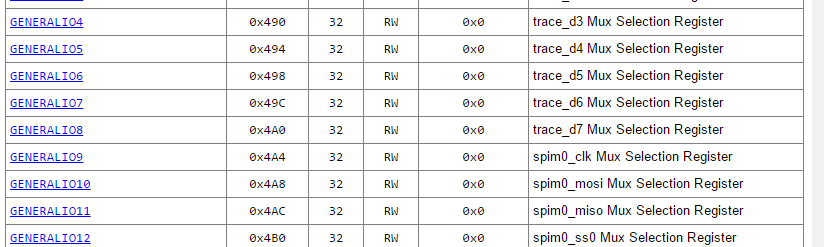
\includegraphics[scale = 0.8]{figures/fig_pinmuxregisters_doc.png}
\end{center}
\caption{Consulting the Cyclone V HPS Memory Map for the list of Pin Mux Control registers.}
\label{fig:pinmuxregisters_doc}
\end{figure}

By clicking on one of the pin multiplexing registers, you can see a list of possible routings that can be made for the corresponding pin. Figure~\ref{fig:generalio7_reg} shows the list for the \textit{GENERALIO7} register (\textit{trace\_d6} pin). Note that the routing options for \textit{trace\_d7} is similar to \textit{trace\_d6}. 

\begin{figure} [H]
\begin{center}
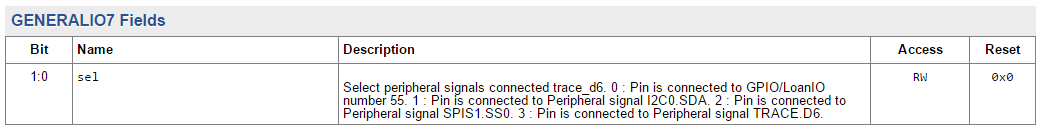
\includegraphics[scale = 0.6]{figures/fig_generalio7_reg.png}
\end{center}
\caption{Consulting the Cyclone V HPS Memory Map for details of the \textit{GENERALIO7} register.}
\label{fig:generalio7_reg}
\end{figure}

\vskip 0.5in
The possible routings for \textit{trace\_d6} are described in more detail below:

\begin{enumerate}
\item GPIO/LoanIO number 55: A value of 0 routes the pin to the GPIO/LoanIO multiplexer, which in turn can route this signal to either the GPIO controller or to the FPGA fabric as a LoanIO wire.
\item I2C0.SDA: A value of 1 routes the pin to SDA port of the I2C controller \textit{I2C0}.
\item SPIS1.SS0: A value of 2 routes the pin to the SS0 port of the SPI Slave controller \textit{SPIS1}.
\item TRACE.D6: A value of 3 routes the pin to the D6 port of the Trace controller. 
\end{enumerate}

Figure~\ref{fig:pinmux} provides a high-level view of the ADXL345's signals, and the multiplexers involved in routing them. The typical routing configuration is to connect the ADXL345's I2C signals to the \textit{I2C0} I2C controller. This allows a master to communicate with the ADXL345 chip via \textit{I2C0}'s memory-mapped register interface. This means writing `1' to \textit{GENERALIO7} and \textit{GENERALIO8}, and `0' to \textit{I2C0USEFPGA}. %a block diagram of the multiplexers involved in routing the ADXL345 signals.  a block diagram that summarizes the possible routing configurations for the ADXL345 connection. shows the multiplexers involved in routing the \textit{trace\_d6} and \textit{trace\_d7} pins inside the HPS. Some of the possible routings and the required register configurations to achieve each routing are shown below:

\begin{figure} [H]
\begin{center}
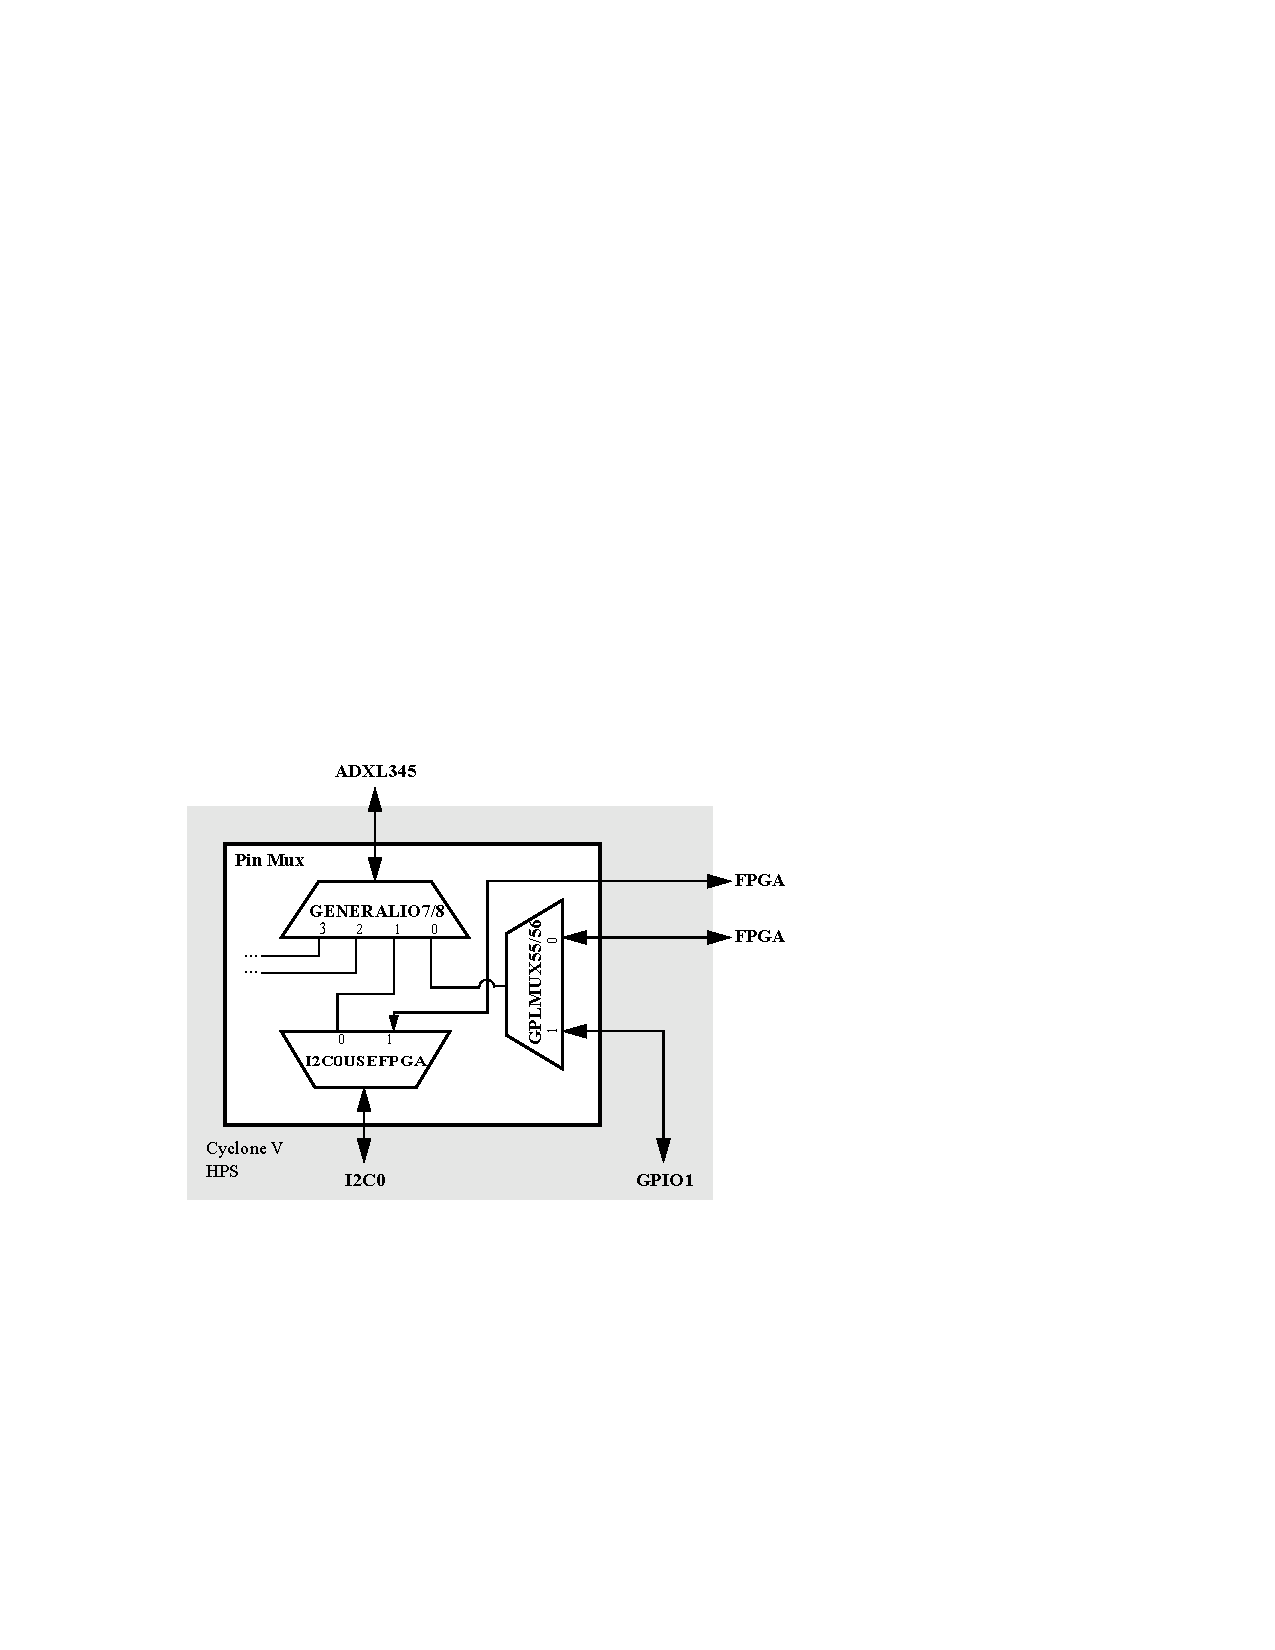
\includegraphics[scale = 0.8]{figures/fig_pinmux.pdf}
\end{center}
\caption{Routing the I2C signals from the accelerometer in a DE1-SoC board.}
\label{fig:pinmux}
\end{figure}

\iffalse
\begin{table}[h]
    \centering
    \begin{tabular}{|c|c|c|c|c|}
        \hline
        \multicolumn{5}{|c|}{\textit{\textbf{Table 2. Example Routing Configurations of the ADXL345 I2C Signals on the DE1-SoC}}}
        \\\hline
            \textbf{Routing Destination}
            & \textbf{GENERALIO7/8}
            & \textbf{GPLMUX55/56}
            & \textbf{I2C0USEFPGA}
            & \textbf{Routing Diagram}
        \\\hline
            I2C0 Controller
            & 1
            & DON'T CARE
            & 0
            & lalala
        \\\hline
            GPIO1 Controller
            & 0
            & 1
            & DON'T CARE
            & lalala
        \\\hline
            FPGA (LoanIO port)
            & 0
            & 0
            & DON'T CARE
            & lalala
        \\\hline
    \end{tabular}
    \label{tab:builtindevices}
\end{table}
\fi


\subsection{Allowing Non-Secure Access to Devices}

The HPS interconnect contains a security feature that limits access to various devices so that only ``secure'' masters, such as the ARM* Cortex* A9 processor, can access them. Because masters in the FPGA are considered non-secure, a secure master must first configure the interconnect to allow non-secure access to a device before FPGA-side masters can access it. This is done by writing to \textit{Security Register Group} registers, which are part of the \textit{L3 GPV Registers}. To allow non-secure access to a device, a `1' must be written to the device's corresponding security bit. For example, to allow non-secure access to \textit{I2C0}'s register interface, you must write a `1' to bit 2 of the \textit{l4sp} register. Further details about the \textit{Security Register Group} registers can be found in the \textit{Cyclone V HPS Memory Map}, as shown in Figure~\ref{fig:securityregs}.

\begin{figure} [H]
\begin{center}
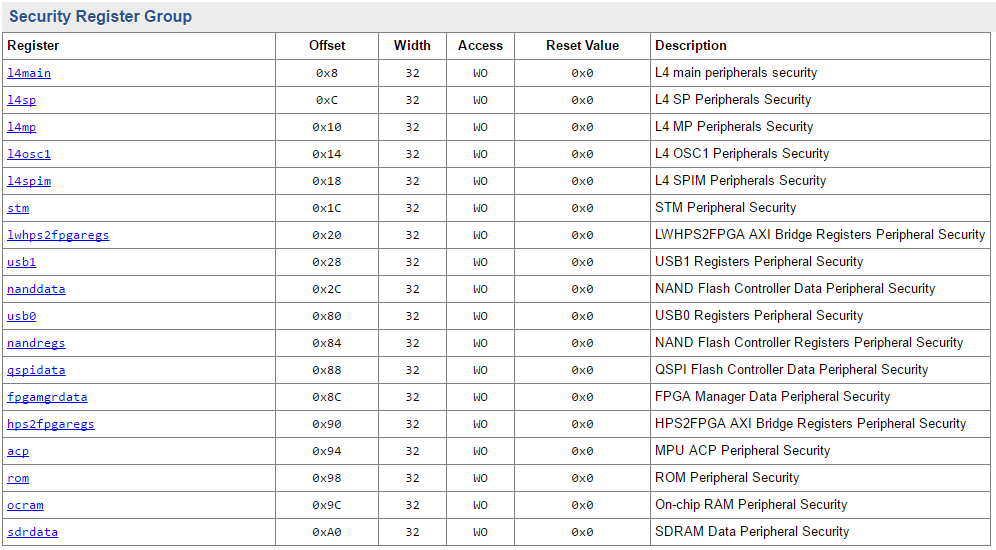
\includegraphics[scale = 0.6]{figures/fig_securityregisters.png}
\end{center}
\caption{The L3 GPV Security Registers, seen in the \textit{Cyclone V HPS Memory Map}.}
\label{fig:securityregs}
\end{figure}

%Connections inside the HPS to these peripheral pins can be
%configured to route the signals to various end points, including routing them to the FPGA fabric, thus giving FPGA-side
%components access to these external devices.

\section{Accessing the HPS Interconnect from the FPGA}

\subsection{Connecting an FPGA Master to the HPS Interconnect}

An AXI or Avalon\textsuperscript{\textregistered} bus-mastering device inside the FPGA can be connected to the HPS interconnect through the FPGA-to-HPS bridge. This connection is
made in the Platform Designer system integration tool, by connecting the master device's memory mapped master port to the \textit{Hard Processor System} component's
AXI\_Slave port named \textit{f2h\_axi\_slave}. Figure~\ref{fig:nios_to_hps} shows an example of such connection in the Platform Designer GUI, where the master device is an instantiation of the Nios\textsuperscript{\textregistered} II soft processor. 
%The connection is made by connecting the \textit{data\_master} port of the Nios II processor to the \textit{f2h\_axi\_slave} port of the Arria V/Cyclone V Hard Processor System.

\begin{figure} [H]
\begin{center}
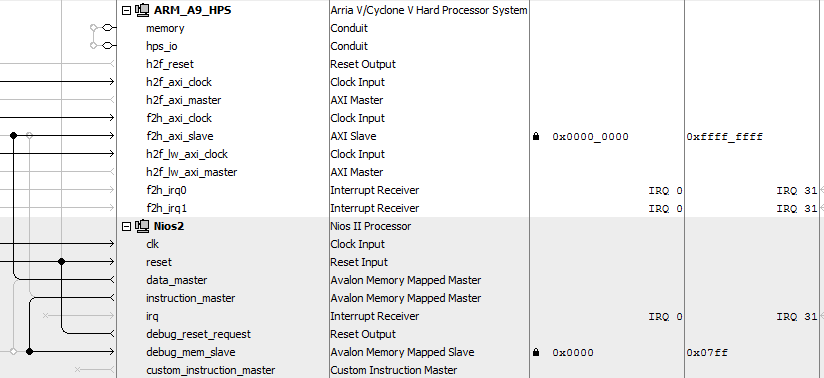
\includegraphics[scale = 0.8]{figures/fig_Nios_to_HPS.png}
\end{center}
\caption{Connecting an FPGA-side master to the HPS interconnect.}
\label{fig:nios_to_hps}
\end{figure}

\subsection{Enabling the FPGA-to-HPS Bridge}

Before FPGA-side masters can access the HPS interconnect, the FPGA-to-HPS bridge must first be enabled by deasserting its reset bit in the \textit{brgmodrst}. The \textit{brgmodrst} register is located at address \texttt{0xFFD0501C} in HPS address space. Since FPGA-side masters cannot access HPS address space until the bridge is enabled, the resets must be deasserted by a master inside the HPS. This is usually accomplished by running a baremetal program on the ARM Cortex A9 processor to write a 0 to bit 2 of the \textit{brgmodrst} register. After deasserting the bridge's reset, the FPGA-side master has access to the full 4GB address space through the FPGA-to-HPS bridge. 

\subsection{The Address Span Extender}

The HPS interconnect has an address space that spans 4GB, which takes up the entirety of a 32-bit master's address range. This scenario was shown in Figure~\ref{fig:nios_to_hps}, where the \textit{f2h\_axi\_slave} connection took up the entire 32-bit (\texttt{0x00000000} - \texttt{0xffffffff}) address range of the Nios II processor. Such a connection would prevent the master from addressing any other memory-mapped device. As a workaround to this limitation, you can use a standard Platform Designer IP core called the \textit{Address Span Extender}.

The \textit{Address Span Extender} IP core provides a window into the address space of a slave. Figure~\ref{fig:nios_to_hps_via_addr_extender} shows the use of the \textit{Address Span Extender} to provide a 16MB window into the top portion of the HPS interconnect's memory range, from 0xFF000000 to 0xFFFFFFFF. This window provides the Nios II processor access to all of the HPS's built-in devices listed in Section~\ref{sec:built_in_devices}, and leaves the rest of the address range free for addressing other memory-mapped devices. The size of the window, as well as the window's offset from the base address of the slave can be configured during the instantiation of the core. For further details regarding the \textit{Address Span Extender}, refer to the \textit{Platform Designer System Design Components } section of the \textit{Quartus\textsuperscript{\textregistered} Prime Handbook}.

\begin{figure} [H]
\begin{center}
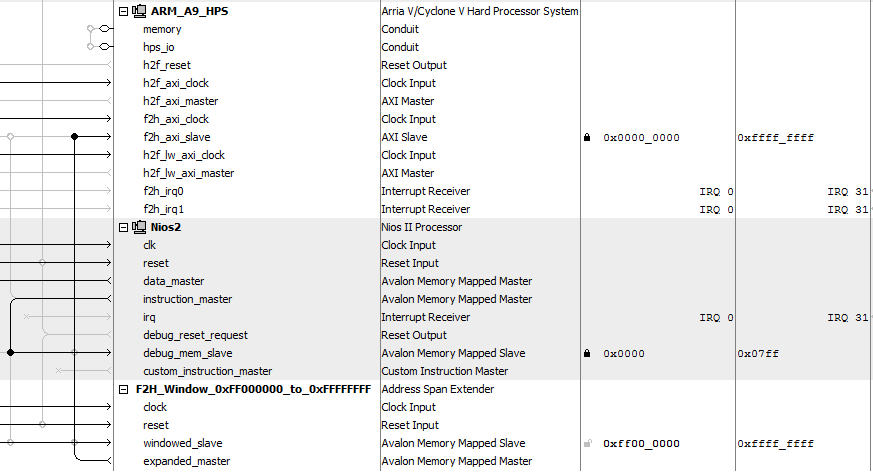
\includegraphics[scale = 0.5]{figures/fig_Nios_to_HPS_via_addr_extender.png}
\end{center}
\caption{Connecting an FPGA-side master to the HPS interconnect via an address span extender.}
\label{fig:nios_to_hps_via_addr_extender}
\end{figure}

\iffalse
\subsection{Cache-Coherent Access via the Accelerator Coherency Port}

TO INCLUDE OR NOT INCLUDE THIS SECTION. THAT IS THE QUESTION.

To access portions of the HPS address range that are cached by the ARM Cortex-A9 processor in a cache-coherent manner, the FPGA master must access the memory through the \textit{Accelerator Coherency Port} (ACP). The portion of memory that is cached includes the main memory (DDR3 SDRAM in most cases). Memory accesses made through the ACP go through the ARM processor's L2 cache, ensuring reads and writes to cached lines are done coherently. The use of the L2 cache also gives potential performance benefit, if accesses result in hits in the cache.

CONFIGURING THE ACP?

\textbf{DIAGRAM OF ACP port, maybe memory span}
\fi

\section{Accessing HPS Peripheral Pins from the FPGA}

This section describes how to connect HPS peripheral pins as input, output, or inout ports to user-defined HDL modules in the FPGA. 

\subsection{Using the LoanIO Interface in Platform Designer}
\label{sec:loanio_qsys}

In Figure~\ref{fig:pinmux} you can see that the pin multiplexing can be configured to route the ADXL345 I2C pins to the FPGA side, by setting \textit{GENERALIO7/8} to '0' and \textit{GPLMUX55/56} to '0'. When the multiplexing is configured in such a way, the pins can be accessed through the \textit{LOANIO} port of the Hard Processor System component in Platform Designer. In order to use the \textit{LOANIO} port, you must first configure the HPS component in the \textit{Peripheral Pins} tab of the component wizard. Near the bottom of the tab, you will see a table of peripheral pins, as shown in Figure~\ref{fig:loanio_table}. In the table, you must export the required pins to the \textit{LOANIO} interface by clicking on the \textit{LOANIOXX} button in the corresponding row. Figure~\ref{fig:loanio_table} shows this being done for the pins \textit{trace\_d6} and \textit{trace\_d7}. 

\begin{figure} [H]
\begin{center}
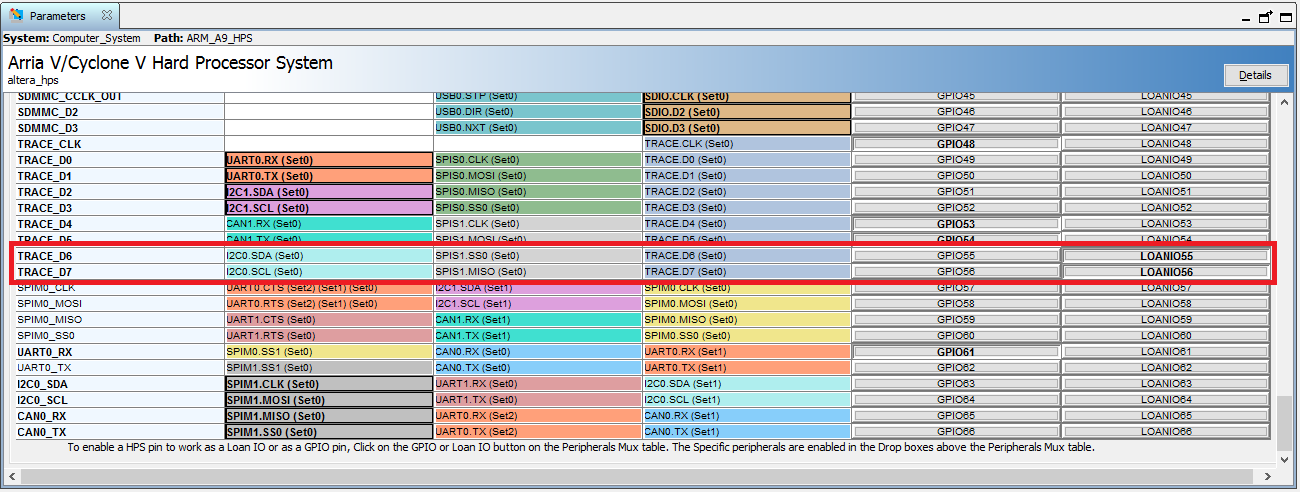
\includegraphics[scale = 0.5]{figures/fig_qsys_hps_loanio.png}
\end{center}
\caption{Configuring the HPS Platform Designer Component to connect HPS peripheral pins to the \textit{LOANIO} port.}
\label{fig:loanio_table}
\end{figure}

Once the HPS component is configured, the HPS component will now have a conduit named \textit{h2f\_loan\_io}, as shown in Figure~\ref{fig:hps_component_loanio_port}. To access this port in your HDL code, you must export it by double clicking the \textit{Double-click to export} text to the right of the \textit{h2f\_loan\_io} conduit. This will result in three additional ports in the top-level module generated by Platform Designer, as shown in Figure~\ref{fig:exported_loanio}. These ports are as wide as the number of HPS peripheral pins that exist in the chip. In the case of the DE1-SoC board, the ports are 67 bits wide corresponding to the 67 HPS peripheral pins. In Figure~\ref{fig:loanio_table}, you can see that the two pins that we exported are sent to \textit{LOANIO55} and \textit{LOANIO56}, meaning that the two pins can be accessed at indices 55 and 56 in the three ports. 

\begin{figure} [H]
\begin{center}
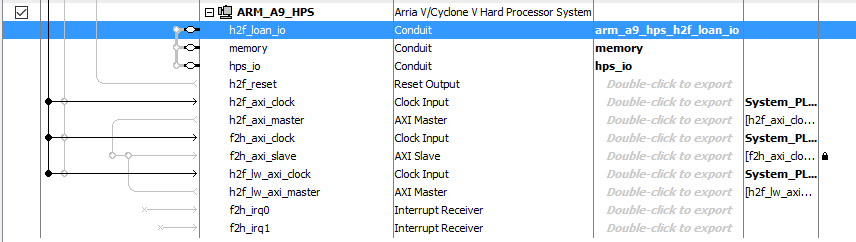
\includegraphics[scale = 0.7]{figures/fig_qsys_loanio_export.png}
\end{center}
\caption{Exporting the HPS component's \textit{LOANIO} port.}
\label{fig:hps_component_loanio_port}
\end{figure}

\begin{figure} [H]
\begin{center}
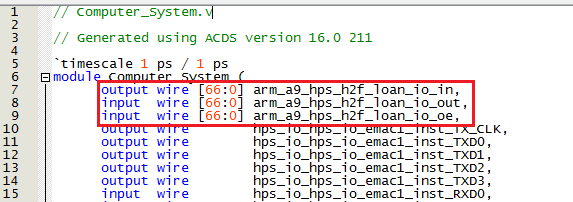
\includegraphics[scale = 0.7]{figures/fig_exported_loanio.png}
\end{center}
\caption{The exported \textit{LOANIO} port.}
\label{fig:exported_loanio}
\end{figure}

\subsection{Configuring Pin Multiplexing for LoanIO}

Section~\ref{sec:loanio_qsys} described the FPGA-side configuration for using the \textit{LOANIO} port. HPS-side configuration for using the \textit{LOANIO} port is done in a similar way as described in Section~\ref{sec:pinmuxing}. The goal is to configure the pin multiplexers to route the pins to the \textit{LOANIO} port. First, the \textit{GENERALIO} multiplexer corresponding to the pin must be configured to '0' to route the pin to the \textit{GPIO/LOANIO} interface. Then, the corresponding \textit{GPLMUX} multiplexer must be configured to '0', which routes the pin to the \textit{LOANIO} port. 

%\subsection{Setting Up an ARM SD Card for Automatic Pin Multiplexer Configuration}

%Use Academic Monitor Program to develop a baremetal program that configures pin multiplexers then create the SD card.



\clearpage

\vspace{1in}
% Copyright and Trademark

%\newcommand{\datePublished}{Mar 2022}

\newcommand{\versnum}{21.1} %version number quartus/AMP
\newcommand{\quartusname}{Quartus\textsuperscript{\textregistered} Prime}	
\newcommand{\textBar}{For \quartusname{} \versnum{}}
\newcommand{\thisyear}{2022 } %for copyright
\newcommand{\company}{FPGAcademy.org}
\newcommand{\longteamname}{FPGAcademy.org}
\newcommand{\teamname}{FPGAcademy}
\newcommand{\website}{FPGAcademy.org}

\newcommand{\productAcronym}{AMP}
\newcommand{\productNameShort}{Monitor Program}

\newcommand{\productNameMedTM}{Monitor Program}
\newcommand{\productNameMed}{Monitor Program}

%\newcommand{\headerLogoFilePath}[1]{#1/FPGAcademy.png}



%%%%%%%%%%%%%%%%%%%%%%%%%%%%%%%%%%%%%%%%
%%% FPGAcademy Copyright Information %%%
%%%%%%%%%%%%%%%%%%%%%%%%%%%%%%%%%%%%%%%%

%Always put the copyright on a new page (clear page), with some vertical space from top
\clearpage
\vspace{1in}

\noindent

Copyright {\copyright} FPGAcademy.org. All rights reserved. FPGAcademy and the FPGAcademy logo are trademarks of  FPGAcademy.org.  This document is being provided on an ``as-is'' basis and as an accommodation and therefore all warranties, representations or guarantees of any kind (whether express, implied or statutory) including, without limitation, warranties of merchantability, non-infringement, or fitness for a particular purpose, are specifically disclaimed.

%FPGAcademy assumes no responsibility or liability arising out of the application or use of any information,  product,  or  service  described  herein  except  as  expressly  agreed  to  in  writing  by  FPGAcademy.



**Other names and brands may be claimed as the property of others.




\end{document}

